\documentclass{llncs}

\usepackage[noend]{algpseudocode}
\usepackage{subcaption}
\usepackage{subfig} 
\usepackage{usual}
\usepackage{graphicx}
\pagestyle{plain}
\usepackage{color}


%
\begin{document}
\title{Agent utterances in the dialogue}
\maketitle 

The dialogue model constructed so far allows the user to choose any utterance of the five modeled utterances at each speaking slot. For this reason, The agent has to be able de to respond consistently regardless to the utterance chosen by the user. In this report, I present my model of utterances responses that the agent can choose for each type of received utterance. This model take in account the current mental state when the user utterance was received and its perception of the relationship. We focus on the relation of dominance that takes three values: \{Dominant, submissive, peer\}.

\par In the following, I present the agent possible responses for each utterance. 
\section{State Preference (C, less, more)}
\begin{figure}[b]
	\centerline{\includegraphics[width=5in]{utterances/StatePref.pdf}}
	\vskip 8pt
	\defig{state}{agent possible answers to a state Preference}
\end{figure}

	\par A user can state a preference on values of a certain criterion \emph{C}. As explained, the semantic of the utterance allows the speaker to express three different cases:
	\begin{itemize}
		\item StatePreference(C, less, more) : I like "less" less than "more"
		\item StatePreference(C, *, more): I like the most More
		\item StatePreference(C, less, *): I like the least less. 
	\end{itemize}
	
	\par The agent analyses the values of the received utterance. First, the agent checks that its last utterance is not a ``StatePreference'' about the expressed values, which is done with the method \emph{isTheSameStatement}. The algorithm of this method is depicted bellow: 
	
	\begin{figure}[h]
		
		\begin{algorithmic}[1]\small
			
			\Procedure{isTheSameStatement}{$(less, more)$}

			\State $lastAgentUtt\gets$ $getLastAgentUtterance() $
			\State $lastUserUtt\gets$ $getLastUserUtterance() $
			\If{$(lastAgentUtt == null)$ and $(lastUserUtt == null)$} return $false$
			\EndIf
			\If{$(lastAgentUtt.getMore() == null$)}
				\If{$lastAgentUtt.getLess() == lastUserUtt.getLess()$ or 
				 $lastAgentUtt.getLess() == lastUserUtt.getMore()$}
					return $true$
				\EndIf
			\EndIf
			
			\If{$(lastUserUtt.getMore() == null$)}
				\If{$lastUserUtt.getLess() == lastAgentUtt.getLess()$ or 
				$lastUserUtt.getLess() == lastAgentUtt.getMore()$}
			return $true$
				\EndIf
			\EndIf
			
			\If{$(lastAgentUtt.getLess() == null$)}
				\If{$lastAgentUtt.getMore() == lastUserUtt.getLess()$ or 
				$lastAgentUtt.getMore() == lastUserUtt.getMore()$}
			return $true$
				\EndIf
			\EndIf
			
			
			\If{$(lastUserUtt.getLess() == null$)}
				\If{$lastUserUtt.getMore() == lastAgentUtt.getLess()$ or 
					$lastUserUtt.getMore() == lastAgentUtt.getMore()$}
				return $true$
				\EndIf
			\EndIf
			\EndProcedure
	  \end{algorithmic}
	  \vskip 8pt
	  \defig{pseudo}{Pseudocode for hybrid reactive HTN execution and recovery system.}
	\end{figure} 
	
	to and depending on the perception of the relationship, the agent will choose  an adequate answer. The possibles responses are depicted in \fig{state}, and explained in the following: 
	\begin{enumerate}
{ \color{red}		\item \textbf{StatePreference (C, less, more)}:The agent can react to the the stated values by observing its preferences on the stated criteria. This utterance is selected if the agent's previous utterance doesn't concern a statement about (less, more). 
		The condition "sameStatement" is computed with the following algorithm: 
		
		This condition avoid the agent to fall in infinite loop.  Depending on the values of the input preference, the agent will respond with one the the following values. 
			\subitem input: \textit{(*, more)} $\rightarrow$ 
				output: \textit{(more, mostPreferred)} if \textit{more $\not = $ mostPreffered,} else \textit{(*, more)}.
			\subitem input: \textit{(less, *)} $\rightarrow$ 
				output: \textit{(leastPreferred,less)} if \textit{less $\not = $ leastPreffered,} else \textit{(less, *)}.
			\subitem input: \textit{(less, more)} $\rightarrow$ Output:  \textit{(less, more)} if(score(less) $<$ score(more)), \textit{else (more,less)}.
	}	
		\item \textbf{StatePreference (C, less1, more1)}: The agent can state a preference about other values than expressed in the user utterance provided that the agent is not submissive. In the case of all the preferences related to the criterion \emph{C} are already expressed (all the preferences are in OAS). The agent expresses a preference about another criterion \emph{C1} such that $\emph{C} \not = \emph{C1}$.
		
		\item \textbf{AskPreference(C, less1, more1)}: THis response is chosen in the case where the agent is submissive so he doesn't want to propose new values. Therefore, he uses the utterance ask to invite the user to choose values. In the same way as the previous responses, if the agent is aware of all the user preferences about the criterion \emph{C}, he will ask the user about his preferences about another criterion \emph{C1}.
		
		
		\item  \textbf{Propose(C, more)}: the choice of the propose utterance depends on the perception of the relationship of dominance : 
			\subitem if the agent is not submissive; then  the value "more" of the expressed preference has to match the most preferred value of the agent preferences on the criterion \emph{C} \textit{(i.e more = mostPreferred)}. Thus, the agent constructs a proposal that takes as value its mostPreferred value of  \emph{C}.
			\subitem If the agent is submissive, he prioritizes the user preferences. Thus, if the statement is of the type (StatePreference (*, more)). The agent proposes to choose the value "more" for \emph{C}.
	\end{enumerate}

\section{Ask Preference (C, less, more)}
	\begin{figure}
		\centerline{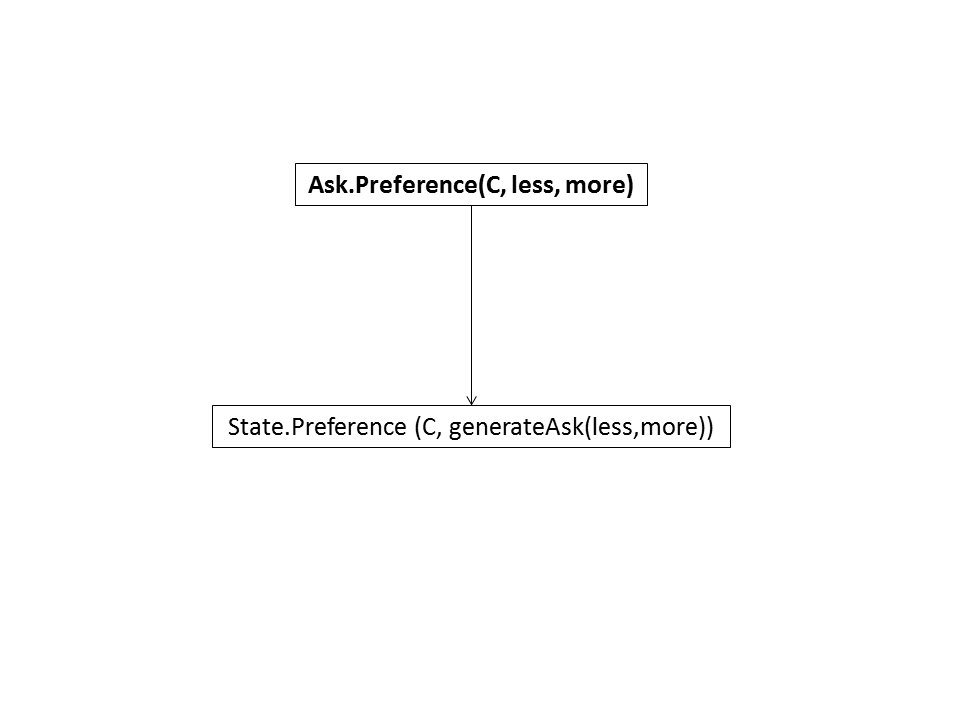
\includegraphics[width=5in]{utterances/Diapositive1.PNG}}
		\vskip 8pt
		\defig{ask}{agent possible answers to an ask Preference}
	\end{figure}
	\par In the case of user asks the agent about a certain preference. The only possible response is to express its opinion about the asked preference.  The content of the response is generated using a method that calculates the values from the input of the ask utterance. We distinguish the following cases, illustrated in \fig{ask}:
		\begin{enumerate}
			\item If \textit{(C, less, more)=(*,*)} thus \textit{reactToAsk(C,less,more) = mostPreferred(C)}. The agent express its most preferred value of the criterion \emph{C}.
				\subitem \textbf{For example :} 
				\subitem U: what kind of cuisine do you prefer ?
				\subitem A: I like Japanese cuisine. (which corresponds to the agent mostPreferred value for the criterion \textit{Cuisine}).
 
			\item  If \textit{(less=*)} and \textit{(more $\not =$ *)}, thus \textit{reactToAsk(*,more)=(*,more) } if \textit{(more=mostPreferred)}, else \textit{reactToAsk(*,more)=(*,mostPreferred)}.
			\subitem For example : 
				\subitem U: Do you like Chinese cuisine ?
				\subitem A: I like Chinese less than Japanese cuisine. (which corresponds to the agent mostPreferred value for the criterion \textit{Cuisine}).
			\item In the same idea, if \textit{(more=*)} and \textit{(less $\not =$ *)}, thus \textit{reactToAsk(less,*)=(less,*)} if \textit{(less=leastPreferred)}, else \textit{reactToAsk(less,*)=(leastPreferred,*)}.
			
		\end{enumerate}

\section{Propose (value)}
	\par When the agent receive a proposal, he can either accept it or reject this proposal. However, we model different ways to express the rejection of a proposal that is influenced by the perception of the relationship. The value of proposal can be either a criterion or an option. (see \fig{prop})
	\begin{figure}[h]
		\centerline{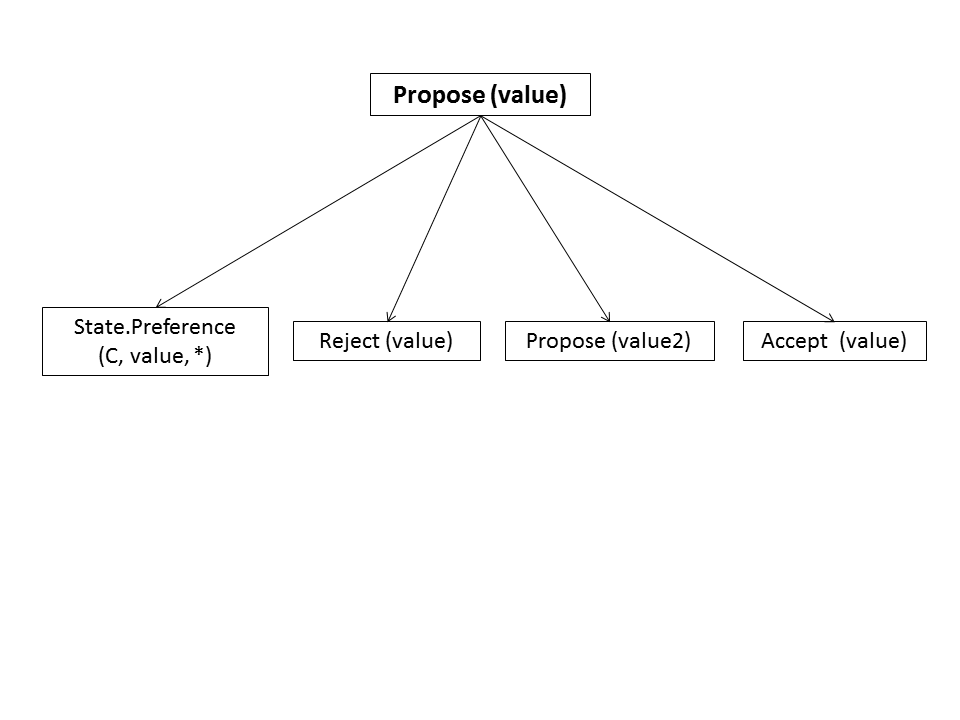
\includegraphics[width=5in]{utterances/Diapositive3.PNG}}
		\vskip 8pt
		\defig{prop}{agent possible answers to a propose utterance}
	\end{figure}
		\begin{enumerate}
			
			\item \textbf{Accept(value)}: A proposal is accepted by the agent only if its score of preference is acceptable. To calculate the acceptance of a proposal, we modeled a simple method that checks if  the score of the value of proposal is acceptable. In the case of a criterion proposal  preference if the score of a criterion is positive then it is acceptable. While options are sorted by their utility rate, and an option is acceptable if its rank in the list is bellow the middle.  Note that, when an option is accepted, the negotiation is closed. 
			
			\item \textbf{Reject(value)}: We suppose that a submissive person is not comfortable with expressing a clear reject. Therefore, we decide that only a non submissive agent can express a reject if the proposed values are not acceptable. 
		
			\item \textbf{StatePreference(C,value,*)}: a submissive agent can express an implicit reject using a statePreference. In the case of a criterion proposal, the proposed value is assigned to the less argument of the preference and the more is calculated from the preference base of the agent, such that $more \notin Rejected$. In the case of option, we extract the criterion that gets the worst score and we generate a preference in the same way than the criterion proposal.
			
			\item \textbf{Propose(value 2)} : This utterance is defined to allow the agent to counter propose another value if the value proposed by the user is not acceptable. This utterance is allowed only for a non submissive agent such that $value2 \not = value$ and $value2 \notin Rejected$. This value can either be a criterion or an option.
	\end{enumerate}
	
\section{Reject (value)}
\par A user can reject a proposal that he doesn't like. Thus, the agent has to react in order to either propose other values or to collect more knowledge about the user preferences. However we defined an additional case for the dominant agent. (see \fig{reject})
\begin{figure}
	\centerline{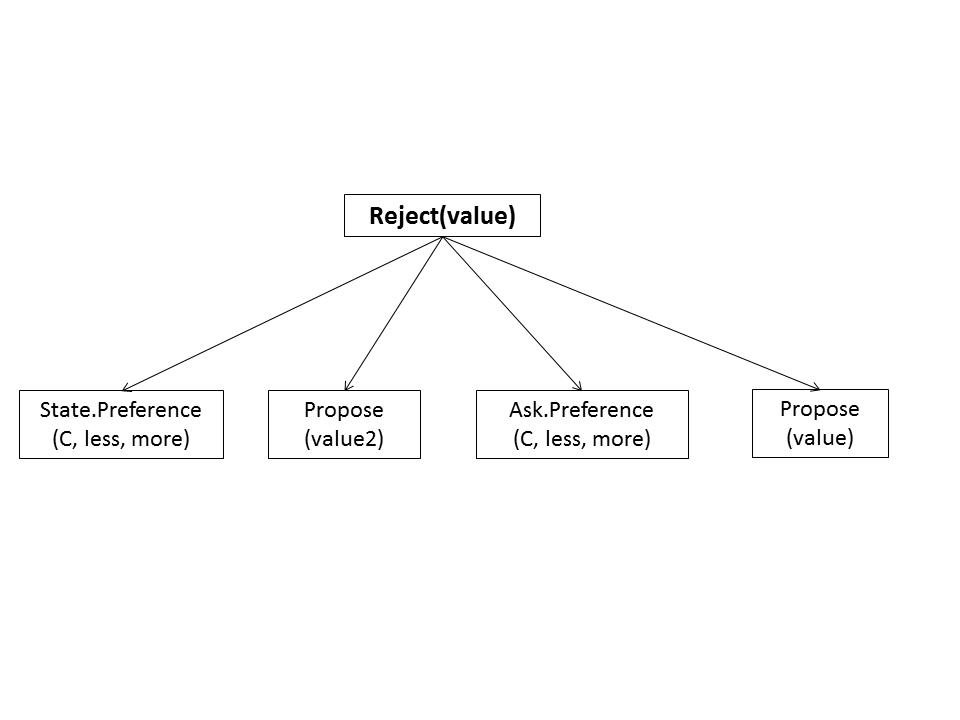
\includegraphics[width=5in]{utterances/Diapositive4.PNG}}
	\vskip 8pt
	\defig{reject}{agent possible answers to reject utterance}
\end{figure}
\begin{enumerate}
	 
	\item \textbf{Propose(value 2)} : if the agent is not submissive, he can propose another proposal which can be either a criterion or an option. The proposed value concerns its most preferred value. The current most preferred value is calculated by taking into account the current state of negotiation (its ignores the rejected criteria and options).
	\item \textbf{AskPreference(C,less,more)}: if the agent is submissive and receives a reject, he would gather more knowledge about the user preferences. Therefore, he'll ask the user about a preference that doesn't exist in other preferences. 
	
	
	\item \textbf{StatePreference(C,less,more)}: The agent continues the negotiation and express its preference concerning the current discussed criterion before the reject.
	
	\item \textbf{Propose(value)}: When the agent is dominant and the rejected value is its most preferred value, we modeled a case where the agent will counter propose with the rejected proposal until the user accepts it. 
			 
\end{enumerate}	

\section{Accept (value)}
\par When a user accept proposal, the agent response will depends on the content of the utterance. If the value is an option, then the negotiation is over and the agent has to close the dialogue. Otherwise, the agent has to open a negotiation on the other criteria, or propose an option that contains the accepted criterion.  In the following, we present the possible responses for an accept value where a value concerns a criterion. 
\begin{figure}[h]
	\centerline{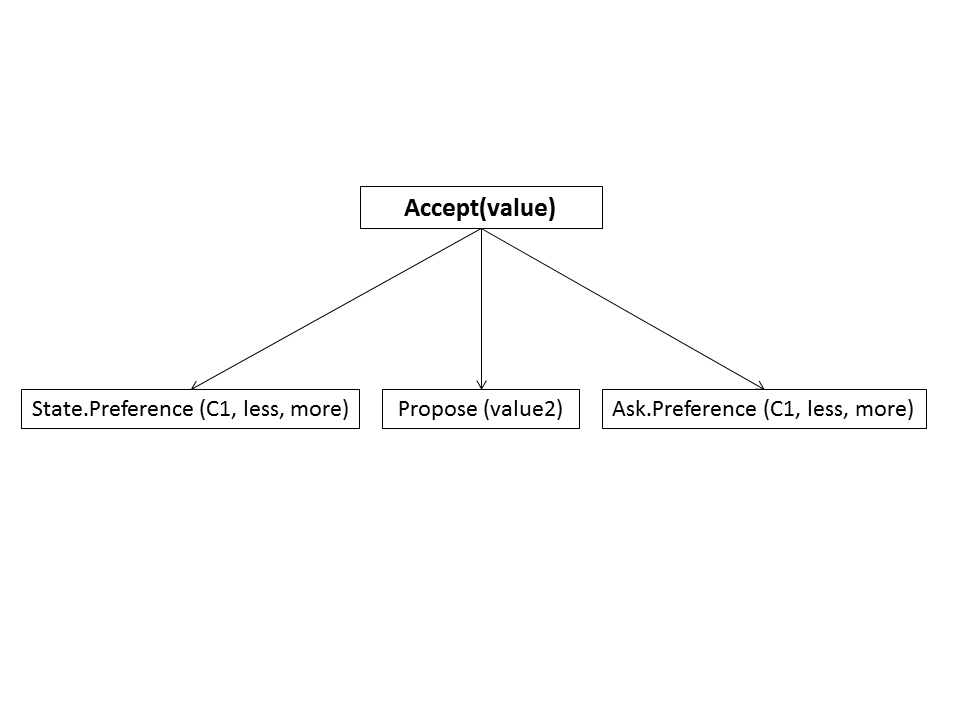
\includegraphics[width=5in]{utterances/Diapositive5.PNG}}
	\vskip 8pt
	\defig{state}{agent possible answers to a accept utterance}
\end{figure}
\begin{enumerate}
	
	\item \textbf{Propose(value 2)} : if the agent is  dominant, he can open a negotiation on an other criterion, by proposing a value. 
	 
	\item \textbf{AskPreference(C1,less,more)}: if the agent is submissive, he would open a new negotiation by asking the user his preferences about the criterion \emph{C1}, where type(value) $not=$  \emph{C1}.
	
	
	\item \textbf{StatePreference(C1,less,more)}: The agent continues the negotiation and express its preference concerning the new discussed criterion.
	
\end{enumerate}	

	\par This propositions remain a first test and ameliorations will be proposed soon.

\end{document}